\section{Evaluation}
\label{sec:results}

This section evaluates the characteristics of the BlueDBM implementation.

\subsection{FPGA Resource Utilization}

The FPGA resource usage of each of the two Artix-7 chips are shown in
Table~\ref{tab:artixutil}. 46\% of the I/O pins were used either to communicate
with the FMC port or to control the flash chips.

\begin{table}[h]\footnotesize
\centering
\begin{tabular}{l | c | c | c | c |}
Module Name & \# & LUTs & Registers & BRAM \\
\hline \hline
Bus Controller & 8 & 7131 & 4870 & 21 \\
$\rightarrow$ ECC Decoder & 2 & 1790 & 1233 & 2 \\
$\rightarrow$ Scoreboard & 1 & 1149 & 780 & 0 \\
$\rightarrow$ PHY & 1 & 1635 & 607 & 0 \\
$\rightarrow$ ECC Encoder & 2 & 565 & 222 & 0 \\
\hline
SerDes & 1 & 3061 & 3463 & 13 \\
\hline \hline
\multicolumn{2}{c}{
Artix-7 Total
} & 75225 (56\%) & 62801 (23\%) & 181 (50\%)
\end{tabular}
\caption{Flash Controller on Artix 7 Resource Usage}
\label{tab:artixutil}
\end{table}

The FPGA resource usage of the Virtex 7 FPGA chip on the VC707 board is shown in
Table~\ref{tab:virtexutil}. As it can be seen, there is still enough space for accelerator development on the Virtex FPGA.



\begin{table}[h]\footnotesize
\centering
\begin{tabular}{l | c | c | c | c | c |}
Module Name & \# & LUTs & Registers & RAMB36 & RAMB18 \\
\hline \hline
Flash Interface & 1 & 1389 & 2139 & 0 & 0 \\
Network Interface& 1 & 29591 & 27509 & 0 & 0\\
DRAM Interface& 1 & 11045 & 7937 & 0  & 0\\
Host Interface& 1 & 88376 & 46065 & 169 & 14 \\
\hline \hline
\multicolumn{2}{c}{
Virtex-7 Total
} & 135271& 135897 & 224 & 18 \\
\multicolumn{2}{c}{
} & (45\%) & (22\%) & (22\%) & (1\%)
\end{tabular}
\caption{Host Virtex 7 Resource Usage}
\label{tab:virtexutil}
\end{table}


\subsection{Power Consumption}
Table~\ref{tab:power} shows the overall power consumption of the system, which
were estimated using values from the datasheet. Thanks to the low power
consumption of the FPGA and flash devices, BlueDBM does not add much power
consumption to the system.

\begin{table}[h]\footnotesize
\centering
\begin{tabular}{l | r}
Component & Power (Watts) \\
\hline \hline
VC707 & 30 \\
Flash Board x2 & 10 \\
Xeon Server & 200 \\
\hline
Node Total & 240 \\

\end{tabular}
\caption{BlueDBM Estimated Power Consumption}
\label{tab:power}
\end{table}

\begin{figure*}[ht]
\centering
\vspace{0pt}
\begin{minipage}[c]{.3\textwidth}
	\includegraphics[width=0.27\paperwidth]{graphs/obj/network-crop.pdf}
	\caption{BlueDBM Integrated Network Performance}
	\label{fig:result_network}
\end{minipage}\hfill
\vspace{0pt}
\begin{minipage}[c]{.3\textwidth}
	\includegraphics[width=0.27\paperwidth]{graphs/obj/latency-crop.pdf}
	\caption{Latency of Remote Data Access in BlueDBM}
	\label{fig:result_latency}
\end{minipage}\hfill
\vspace{0pt}
\begin{minipage}[c]{.3\textwidth}
	\includegraphics[width=0.27\paperwidth]{graphs/obj/bandwidth-crop.pdf}
	\caption{Bandwidth of Data Access in BlueDBM}
	\label{fig:result_bandwidth}
\end{minipage}
\end{figure*}

\subsection{Network Performance}

We measured the performance of the network by transferring a single stream of 128 bit data packets through multiple nodes across the network in a non-contentious traffic setting. The maximum physical link bandwidth is 10Gbps, and per-hop latency is 0.48 $\mu s$.
Figure~\ref{fig:result_network} shows that we are able to sustain 8.2Gbps of bandwidth per stream across multiple network hops. This shows that the protocol overhead is under 18\%. The latency is 0.48 $\mu s$ per network hop, the end-to-end latency is simply a multiple of network hops to the destination. 

Each node in our BlueDBM implementation includes a fan-out of 8 network
ports, so each node can have an aggregate full duplex bandwidth of 8.2GB/s. With
such a high fan-out, it would be unlikely that a remote node in a rack-class
cluster to be over 4 hops, or 2 $\mu s$ away. Even if we assume a naive ring
network of 20 nodes with 4 lanes each to next and previous nodes, the average
latency to a remote node would be 2.5 $\mu s$, with the ring throughput of 32.8
Gbps. \emph{Assuming a flash access latency of 50 $\mu s$, such a network will only add 5\% latency in the worst case, giving the illusion of a uniform access storage.}


%\begin{figure}[h]
%	\begin{center}
%	\includegraphics[width=0.3\paperwidth]{graphs/obj/network-crop.pdf}
%	\caption{BlueDBM Integrated Network Performance}
%	\label{fig:result_network}
%	\end{center}
%\end{figure}

\subsection{Remote Storage Access Latency}
\label{sec:latency}

We measured the latency of remote storage access by reading an 8K page of data from the following sources using the integrated storage network: 

\begin{enumerate}
\item ISP-F: From in-store processor to remote flash storage;
\item H-F: From host server to remote flash storage;
\item H-RH-F: From host server to remote flash storage via its host server.
\item H-D: From host server to remote DRAM; 
\end{enumerate}

In each case, the request is sent from either the host server or the in-store processor on the local BlueDBM node. In the third and fourth case, the request is processed by the remote server, instead of the remote in-store processor, adding extra latency. However, data is always transferred back via the integrated storage network. We could have also measured the accesses to remote servers via Ethernet, but that latency is at least 100x of the integrated network, and will not be particularly illuminating.

\begin{figure}[b]
	\centering
	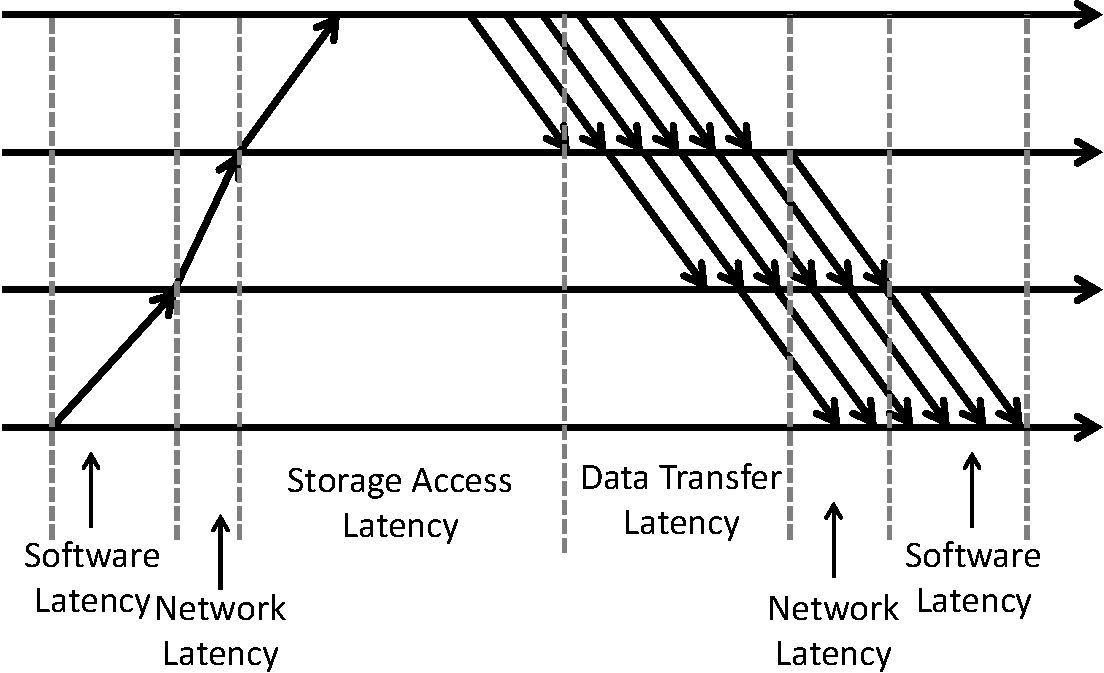
\includegraphics[width=0.40\textwidth]{figures/latencybreak-crop.pdf}
	\caption{Breakdown of Remote Storage Access Latency}
	\label{fig:latencybreak}
\end{figure}

The latency is broken up into four components as shown in Figure~\ref{fig:latencybreak}. First is the local software overhead of accessing the network
interface. Second is the storage access latency, or the time it takes for the
first data byte to come out of the storage device. Third is the amount of times
it takes to transfer the data until the last byte is sent back over the network,
and last is the network latency.

Figure~\ref{fig:result_latency} shows the exact latency breakdown for each experiment. Notice in all 4 cases, the network latency is insignificant. The data transfer latency is similar except when data is transferred from DRAM (H-D), where it is slightly lower. Notice that except in the case of ISP-F, storage access incurs the additional overhead of PCIe and host software latencies. If we compare ISP-F to H-RH-F, we can see the benefits of an integrated storage network, as the former allows overlapping the latencies of storage and network access. 

%\begin{figure}[h]
%	\begin{center}
%	\includegraphics[width=0.3\paperwidth]{graphs/obj/latency-crop.pdf}
%	\caption{Latency of Data Access in BlueDBM}
%	\label{fig:result_latency}
%	\end{center}
%\end{figure}
%Latency for 
%
%fpga<-> flash
%fpga<-> remote flash
%
%host<-> flash
%host<-> remote flash
%host<-> remote host DRAM
%fpga<-> remote ssd using samsung...


\subsection{Storage Access Bandwidth}

We measured the bandwidth of BlueDBM by sending a stream of millions of random read requests for 8KB size pages to local and remote storage nodes, and measuring the elapsed time to process all of the requests.
We measured the bandwidth under the following scenarios:
\begin{enumerate}
\item Host-Local: Host sends requests to the local flash and all data is streamed returned over PCIe;
\item ISP-Local: Host sends requests to the local flash and all data is consumed at the local in-store processor;
\item ISP-2Nodes: Like ISP-Local except 50\% of the requests are sent to a remote flash controller. Only one serial link connects the two nodes;
\item ISP-3Nodes: Like ISP-Local except 33\% of the requests are sent to each of the two remote flash controllers. Two serial links connect each remote controller to the local controller.
\end{enumerate}

Figure~\ref{fig:result_bandwidth} shows the read bandwidth performance for each of these cases. Our design of the flash card provides 1.2GB/s of bandwidth per card. Therefore in theory, if both cards are kept completely busy 2.4GB/s should be the maximum sustainable bandwidth from the in-store processor, and this is what we observe in the ISP-Local experiment. In our Host-Local experiment, we observed only 1.6GB/s of bandwidth. This is because this is the maximum bandwidth our PCIe implementation can sustain. In ISP-2Nodes, the aggregate bandwidth of two flash devices should add up to 4.8GB/s, but we only observe about 3.4GB/s, because remote storage access is limited by the single 8Gbps-serial link. In ISP-3Nodes, the aggregate bandwidth of three flash devices should add up to 7.2GB/s, but we only observe about 6.5GB/s because the aggregate bandwidth of the four serial links connecting the remote controllers is limited to 32.8Gbps (=4.1GB/s).

What these sets of experiments show is that in order to make full use of flash storage, some combination of fast networks, fast host connections and low software overhead is necessary. These requirements can be somewhat mitigated if we make use of in-store computing capabilities, which is what we discuss next.

%\begin{figure}[h]
%	\begin{center}
%	\includegraphics[width=0.3\paperwidth]{graphs/obj/bandwidth-crop.pdf}
%	\caption{Bandwidth of Data Access in BlueDBM}
%	\label{fig:result_bandwidth}
%	\end{center}
%\end{figure}


